\documentclass[submit]{../harvardml}
\usepackage{../common}

\course{CS1810-S26}
\assignment{Homework \#2}
\duedate{February 27, 2026 at 11:59 PM}

\usepackage[OT1]{fontenc}
\usepackage[colorlinks,citecolor=blue,urlcolor=blue]{hyperref}
\usepackage{graphicx}
\usepackage{subcaption}
\usepackage{fullpage}
\usepackage{amsmath}
\usepackage{todonotes}
\usepackage{amssymb}
\usepackage{framed}
\usepackage{color}
\usepackage{soul}
\usepackage{todonotes}
\usepackage{listings}
\usepackage{enumitem}
\usepackage{bm}
\usepackage{bbm}


\newcommand{\B}{\text{B}}
\newcommand{\Beta}{\text{Beta}}

\usepackage[mmddyyyy,hhmmss]{datetime}

\definecolor{verbgray}{gray}{0.9}

\lstnewenvironment{csv}{%
  \lstset{backgroundcolor=\color{verbgray},
  frame=single,
  framerule=0pt,
  basicstyle=\ttfamily,
  columns=fullflexible}}{}
  

%%%%%%%%%%%%%%%%%%%%%%%%%%%%%%%%%%%%%%%%%%%
%% Solution environment
\usepackage{xcolor}
\newenvironment{solution}{
    \vspace{2mm}
    \color{blue}\noindent\textbf{Solution}:
}{}
%%%%%%%%%%%%%%%%%%%%%%%%%%%%%%%%%%%%%%%%%%%


\begin{document}

\begin{center}
  {\Large Classification and Bias-Variance Trade-offs}\\
\end{center}

\subsection*{Introduction}

This homework is about classification, bias-variance trade-offs, and
uncertainty quantification.

The datasets that we will be working with relate to astronomical observations and loan applicants
The first dataset, found at \verb|data/planet-obs.csv|,
contains information on whether a planet was observed (as a binary
variable) at given points in time. This will be used in Problem 1. The
second dataset, available at \verb|data/hr.csv|, details different
loan applicants and their measured debt to income ratio and credit score. You will
work with this data in Problem 3.

As a general note, for classification problems we imagine that we have
the input matrix $\boldX \in \reals^{N \times D}$ (or perhaps they
have been mapped to some basis $\bm{\Phi}$, without loss of
generality) with outputs now ``one-hot encoded."  This means that if
there are~$K$ output classes, rather than representing the output
label $y$ as an integer~${1,2,\ldots,K}$, we represent $\boldy$ as a
``one-hot" vector of length~$K$. A ``one-hot" vector is defined as
having every component equal to 0 except for a single component which
has value equal to 1.  For example, if there are $K = 7$ classes and a
particular data point belongs to class 3, then the target vector for
this data point would be~$\boldy = [0,0,1,0,0,0,0]$.  We will define
$C_1$ to be the one-hot vector for the 1st class, $C_2$ for the 2nd
class, etc.  Thus, in the previous example $\boldy = C_3$. If there
are $K$ total classes, then the set of possible labels is $\{C_1
  \ldots C_K \} = \{C_k\}_{k=1}^K$.  Throughout the assignment we will
assume that each label $\boldy \in \{C_k\}_{k=1}^K$ unless otherwise
specified. The most common exception is the case of binary
classification ($K = 2$), in which case labels are the typical
integers $y \in \{0, 1\}$.

\subsection*{Resources and Submission Instructions}

% We encourage you to read CS181 Textbook's Chapter 3 for more information on linear classification, gradient descent, and classification in the discriminative setting. Read Chapter 2.8 for more information on the trade-offs between bias and variance.

In problems 1 and 3, you may use \texttt{numpy} or \texttt{scipy}, but not \texttt{scipy.optimize} or \texttt{sklearn}. Example code is given in the provided notebook. In past years, students have reported numerical stability issues for problem 3 and sometimes problem 1; we encourage students to not worry too much about this, as we are mindful of this in grading, but we recommend trying to run your code on \textbf{Google Colab} if you encounter issues (since this has resolved the issue for many students in the past).

Please type your solutions after the corresponding problems using this \LaTeX\ template, and start each problem on a new page. Please submit the writeup PDF to the Gradescope assignment `HW2'. Remember to assign pages for each question. \textbf{You must include any plots in your writeup PDF.} Please submit your \LaTeX file and code files to the Gradescope assignment `HW2 - Supplemental.' The supplemental files will only be checked in special cases, e.g. honor code issues, etc. Your files should be named in the same way as we provide them in the repository, e.g. \texttt{hw2.pdf}, etc.


\newpage
%%%%%%%%%%%%%%%%%%%%%%%%%%%%%%%%%%%%%%%%%%%%%
% Problem 1
%%%%%%%%%%%%%%%%%%%%%%%%%%%%%%%%%%%%%%%%%%%%%

\begin{problem}[Exploring Bias-Variance and Uncertainty, 30pts]
In this problem, we will explore the bias and variance of a few
different model classes when it comes to logistic regression, use cross validation for model selection, and
investigate two sources of predictive uncertainty in a synthetic
(made-up) scenario.

We are using a powerful telescope in the northern hemisphere to gather
measurements of some planet of interest. At certain times however, our
telescope is unable to detect the planet due to its positioning around
its star.  The data in \verb|data/planet-obs.csv| records the
observation time in the ``Time" column and whether the planet was
detected in the ``Observed" column (with the value 1 representing that
it was observed).  These observations were taken over a dark, clear
week, which is representative of the region.  Since telescope time is
expensive, we would like to build a model to help us schedule and find
times when we are likely to detect the planet.

\begin{enumerate}
\item Before we begin fitting any models, let us first derive the mathematical explanation for the bias-variance tradeoff. Let $\mathcal{D}$ denote the training dataset, while $\mathbf{x}$ is a fixed input (not in $\mathcal{D}$). Suppose the labels are generated via $$y = f(\mathbf{x}) + \varepsilon$$ where $f(\mathbf{x})$ is the true regression function and $\varepsilon$ is a noise term with $\mathbb{E}[\varepsilon|\mathbf{x}] = 0$ and $\text{Var}(\varepsilon|\mathbf{x}) = \sigma^2$. We'll denote the predictor learned from $\mathcal{D}$ as $\hat f_\mathcal{D}(\mathbf{x})$. Then, we have the prediction error as $$\text{MSE} = \mathbb{E}_{\mathcal{D}, y|\mathbf{x}}[(y - \hat f_\mathcal{D}(\mathbf{x}))^2]$$ We will see that this error decomposes into a noise term, a bias term, and a variance term. \begin{enumerate}
    \item Show that the expression for MSE above decomposes into $$\mathbb{E}_{y|\mathbf{x}}[(y - f(\mathbf{x}))^2] + \mathbb{E}_\mathcal{D}[(f(\mathbf{x}) - \hat f_\mathcal{D}(\mathbf{x}))^2] + \text{\{third term\}}$$ Hint: Add and subtract $f(\mathbf{x})$.

    \item Show that the third term from our final expression in part (b) simplifies to 0. Hint: Use Adam's Law/Law of Total Expectation.

    \item Show that the first term from our final expression in part (b) represents the noise in our data, i.e. $\mathbb{E}_{y|\mathbf{x}}[(y - f(\mathbf{x}))^2] = \sigma^2$. 

    \item Define the average predictor $\bar f(\mathbf{x}) = \mathbb{E}_\mathcal{D}[\hat f_\mathcal{D}(\mathbf{x})]$. Now show that the the second term from our final expression in part (b) represents the squared bias plus variance, i.e. $\mathbb{E}_\mathcal{D}[(f(\mathbf{x}) - \hat f_\mathcal{D}(\mathbf{x}))^2] = (f(\mathbf{x}) - \bar f(\mathbf{x}))^2 + \mathbb{E}_\mathcal{D}[(\bar f(\mathbf{x}) - \hat f_\mathcal{D}(\mathbf{x}))^2]$. 
\end{enumerate}

  \item Now let's explore the use of different bases to model our data. First, randomly split the data into 10 mini-datasets of size $N = 30$. We will use three different basis functions to model the data. We implemented basis 1 as $[1,t]$, where t is the data to help you get started. Then, choose two basis functions, which you'll use to transform the input data in the regression. (Hint: Examples of such basis functions were given in Lecture 2.) \textbf{Please write your chosen basis functions in the written section of your submission for this part of the question. }
  
  For each of these bases, fit a logistic regression model using sigmoid($\boldw^\top \boldsymbol\phi(t)$) to each dataset by using gradient descent to
        minimize the negative log-likelihood.  This means you will be
        running gradient descent 10 times for each basis, once for each
        dataset.

        Use the given starting values of $\boldw$ and a learning rate of $\eta=0.001$, take 1,000 update
        steps for each gradient descent run, and make sure to average the
        gradient over the data points at each step. These parameters,
        while not perfect, will ensure your code runs reasonably quickly.
  
  \item After consulting with a domain expert, we find that the probability of observing the planet is periodic as the planet revolves around its star---we are more likely to observe the planet when it is in front of its star than when it is behind it. In fact, the expert determines that observation follows the generating process $y \sim \text{Bern}(f(t))$, where $f(t) = 0.4 \times \cos(1.1t + 1) + 0.5$ for $t \in [0, 6]$ and $y \in \{0,1\}$. Note that we, the modelers, do not usually see the true data distribution. Knowledge of the true $f(t)$ is only exposed in this problem to allow for verification of the true bias.

        Use the given code to plot the true process versus your learned models. Include your plots in your solution PDF.

        \textbf{In no more than 5 sentences}, explain how bias and variance are reflected in the 3 types of curves on the graphs.  How do the fits of the individual and mean prediction functions change?  Keeping in mind that none of the model classes match the true generating process exactly, discuss the extent to which each of the bases approximates the true process.


    \item If we were to increase the size of each dataset drawn from $N = 30$ to a larger number, how would the bias and variance change for each basis? Why might this be the case? You may experiment with generating your own data that follows the true process and plotting the results, but this is \textbf{not} necessary. \textbf{Your response should not be longer than 5 sentences}.

    \item Consider the test point $t = 0.1$. Using your models trained on basis $\boldsymbol\phi_3$, report the predicted probability of observation of the \textit{first} model (the model trained on the first 30 data points). How can we interpret this probability as a measure of uncertainty? Then, compute the variance of the classification probability over your 10 models at the same point $t = 0.1$. How does this measurement capture another source of uncertainty, and how does this differ from the uncertainty represented by the classification probability? Repeat this process (reporting the first model's classification probability and the variance over the 10 models) for the point $t = 3.2$.

          Compare the uncertainties and their sources at times $t=0.1$ and $t=3.2$.

    \item We now need to make some decisions about when to request time on
          the telescope.  The justifications of your decisions will be sent to
          your funding agency, which will determine whether you will be
          allocated funds to use the telescope for your project. You seek out a team that has used the alternative telescope
                  for observing this planet, and they provide you their observation
                  file \verb|data/planet-obs-alternate.csv|.
                  Compare the observations from your telescope to theirs.  What
                  seems to be happening?  What might be an appropriate model for
                  this? Your funding agency asks you to refit your models on these
                  new data.  Do you think this is a reasonable ask, and if so, how
                  will it help you make better decisions about when to request
                  viewing time?  If not, why do you think the additional modeling
                  will not help? You do \emph{not} need to do any modeling; answer this question in \textbf{no more than 10 lines}. We are looking for your reasoning; there may be
          more than one valid answer.

  
      \item In part 1, we have selected 3 possible bases to use as features when training a model. This gave us 3 possible models. In this part, we will choose the right learning algorithm by using cross validation. Take your dataset split and train 10 models for each basis, using 9 of the chunks for training and 1 of the chunks for validation. Compare the average error across the 10 folds for the 3 bases. Which basis performs the best? Why do you think it performs the best?    

      
  \end{enumerate}
\end{problem}

\newpage

\begin{solution}
	\begin{enumerate}
    \item \begin{enumerate}
            \item $$\text{MSE} = \mathbb{E}_{\mathcal{D}, y|\mathbf{x}}[(y - \hat f_\mathcal{D}(\mathbf{x}))^2]$$ $$\text{MSE} = \mathbb{E}_{\mathcal{D}, y|\mathbf{x}}[((y - f(x)) + (f(x) - \hat f_\mathcal{D}(\mathbf{x})))^2]$$ $$\text{MSE} = \mathbb{E}_{y|\mathbf{x}}[(y - f(x))^2] + 2\mathbb{E}_{\mathcal{D},y|\mathbf{x}}[(y - f(x))(f(x) - \hat f_\mathcal{D}(\mathbf{x}))] + \mathbb{E}_{\mathcal{D}}[(f(x) - \hat f_\mathcal{D}(\mathbf{x}))^2]$$ $$\text{MSE} = \mathbb{E}_{y|\mathbf{x}}[(y - f(x))^2] + \mathbb{E}_{\mathcal{D}|\mathbf{x}}[(f(x) - \hat f_\mathcal{D}(\mathbf{x}))^2] + \text{\{third term\}}$$
            \item $$2\mathbb{E}_{\mathcal{D},y|\mathbf{x}}[(y - f(x))(f(x) - \hat f_\mathcal{D}(\mathbf{x}))] =$$ $$= 2\mathbb{E}_{\mathcal{D},y|\mathbf{x}}[\epsilon(f(x) - \hat f_\mathcal{D}(\mathbf{x}))]$$ $$= 2\mathbb{E}_{\mathcal{D}}[\mathbb{E}_{y|\mathbf{x}, \mathcal{D}}[\epsilon(f(x) - \hat f_\mathcal{D}(\mathbf{x}))]], \text{using Adam's Law}$$ $$= 2\mathbb{E}_{\mathcal{D}}[\mathbb{E}_{y|\mathbf{x}, \mathcal{D}}[\epsilon](f(x) - \hat f_\mathcal{D}(\mathbf{x}))], \text{since $(f(x) - \hat f_\mathcal{D}(\mathbf{x}))$ is constant given $\mathcal{D}$}$$ $$= 2\mathbb{E}_{\mathcal{D}}[0(f(x) - \hat f_\mathcal{D}(\mathbf{x}))], \text{since $\mathbb{E}[\varepsilon|\mathbf{x}] = 0$}$$ $$= 0$$
            \item $$\mathbb{E}_{y|\mathbf{x}}[(y - f(x))^2] = $$ $$ = \mathbb{E}_{\epsilon|\mathbf{x}}[\epsilon^2]$$ $$ = \text{Var}_{\epsilon|\mathbf{x}} (\epsilon) + (\mathbb{E}_{\epsilon|\mathbf{x}}[\epsilon])^2$$ $$ = \text{Var}_{\epsilon|\mathbf{x}} (\epsilon) + 0$$ $$ = \sigma^2$$
            \item $$\mathbb{E}_{\mathcal{D}|\mathbf{x}}[(f(x) - \hat f_\mathcal{D}(\mathbf{x}))^2] = $$ $$= \mathbb{E}_{\mathcal{D}|\mathbf{x}}[((f(x) - \bar f(\mathbf{x})) + (\bar f(\mathbf{x}) - \hat f_\mathcal{D}(\mathbf{x})))^2]$$ $$= (f(x) - \bar f(\mathbf{x}))^2 + 2\mathbb{E}_{\mathcal{D}|\mathbf{x}}[(f(x) - \bar f(\mathbf{x}))(\bar f(\mathbf{x}) - \hat f_\mathcal{D}(\mathbf{x})) ]+\mathbb{E}_{\mathcal{D}|\mathbf{x}}[(\bar f(\mathbf{x}) - \hat f_\mathcal{D}(\mathbf{x}))^2]$$ $$= (f(x) - \bar f(\mathbf{x}))^2 + 2(f(x) - \bar f(\mathbf{x}))\mathbb{E}_{\mathcal{D}|\mathbf{x}}[(\bar f(\mathbf{x}) - \hat f_\mathcal{D}(\mathbf{x})) ]+\mathbb{E}_{\mathcal{D}|\mathbf{x}}[(\bar f(\mathbf{x}) - \hat f_\mathcal{D}(\mathbf{x}))^2]$$ $$= (f(x) - \bar f(\mathbf{x}))^2 + 2(f(x) - \bar f(\mathbf{x}))(\bar f(\mathbf{x}) - \bar f(\mathbf{x}))+\mathbb{E}_{\mathcal{D}|\mathbf{x}}[(\bar f(\mathbf{x}) - \hat f_\mathcal{D}(\mathbf{x}))^2]$$ $$= (f(x) - \bar f(\mathbf{x}))^2 + 2(f(x) - \bar f(\mathbf{x}))*0+\mathbb{E}_{\mathcal{D}|\mathbf{x}}[(\bar f(\mathbf{x}) - \hat f_\mathcal{D}(\mathbf{x}))^2]$$ $$= (f(x) - \bar f(\mathbf{x}))^2 +\mathbb{E}_{\mathcal{D}|\mathbf{x}}[(\bar f(\mathbf{x}) - \hat f_\mathcal{D}(\mathbf{x}))^2]$$
        \end{enumerate}
        \item basis 2: $[1, t, t^2]$.\\ basis 3: $[1, \text{sin}\ t, \text{cos}\ t]$\\
        \item \ \\
        
\includegraphics[width = 0.5\linewidth]{hw2/img_output/basis1.png}
        
\includegraphics[width = 0.5\linewidth]{hw2/img_output/basis2.png}\\
        \centerline{
\includegraphics[width = 0.5\linewidth]{hw2/img_output/basis3.png}}\\
        Basis 1 has the highest bias, as a linear model is the furthest away from approximating the true process that oscillates, but has a moderate variance, as most individual models are close to the mean model, but there are some outliers.\\
        Basis 2 has lower bias, as the polynomial term is able to capture some curvature, but can't capture the oscillation of the true process. The variance is the biggest here, as we can see that the most models are spread out far from the mean.\\
        Basis 3 has the lowest bias since it can capture the oscillating nature of the true process, but the frequency is off, since our model's basis has a frequency of $t$ but the true process has $1.1t$, so it still has bias. The variance is the lowest, since all models are very close to the mean.\\
        In general, all models are not much better than a random $0/1$ prediction.
        \item The variance would decrease for all 3 bases, as more data points means each individual model is trained on a more representative sample, and so their predictions would agree more, as they would all be closer to the best possible fit for the particular basis. The bias would be unchanged for all bases as no matter how many data points you have, bias can only be changed through having a more expressive model in basis regression.
        \item Classification probabilities for $t = 0.1: 0.496, t = 3.2: 0.486$. Model variances for $t = 0.1: 0.00023, t = 3.2: 0.00036$.\\
        The classification probability is very uncertain at both $t = 0.1$ and $t = 3.2$. This should represent uncertainty in the true process; at those points, it should be equally likely that the planet will be observed or not due to its positioning around the star. This is not true for either of those times though; $t = 3.2$ should be closer to $0.3$, and $t = 0.1$ should be close to $0.7$ as seen in the true model. This is due to the poor performance of the model.\\
        The variance is very low at both $t = 0.1$ and $t = 3.2$, and this low uncertainty is due to the fact that all 10 models agree with each other at those points, so the data is consistent across all folds there.
        \item I plotted how the proportion of observations changes for each of the telescope data. As we can see, for the original telescope, there is a clear periodic pattern, which is what we saw with the true process; the likelihood changes with the position of the planet. The alternative data shows no such pattern; it shows as if there was always ~0.6 chance we will observe planet, no matter its position. So, an appropriate model for that data should be just predict we observe with 60\% probability. It is not a reasonable ask to refit the model to this new data, because it gives us no information about when is a best time to view the planet. This is most likely due to bad conditions of viewing or different location.\\
        
\includegraphics[width = \linewidth]{hw2/img_output/1.6.png}\\
        \item basis1 average error (10-fold): 0.493, basis2 average error (10-fold): 0.367, basis3 average error (10-fold): 0.287. This perfectly agrees with what we saw earlier. The linear model is no better than a random guess, as it's bias is too high. The polynomial model is better, as it can capture the relationship a little better. The third basis is the best as it can capture oscillation, and that's why it's the best. 
	\end{enumerate}
\end{solution}


\newpage
%%%%%%%%%%%%%%%%%%%%%%%%%%%%%%%%%%%%%%%%%%%%%
% Problem 2
%%%%%%%%%%%%%%%%%%%%%%%%%%%%%%%%%%%%%%%%%%%%%

\begin{problem}[Maximum likelihood in classification, 15pts]

Consider now a generative $K$-class model.  We adopt class prior
$p(\boldy = C_k; \bpi) = \pi_k$ for all $k \in \{1, \ldots, K\}$
(where $\pi_k$ is a parameter of the prior).
Let  $p(\boldx|\boldy=C_k)$ denote
the class-conditional density of features $\boldx$ (in this
case for class $C_k$). Consider the data set $\mathcal{D} = \{(\boldx_i, \boldy_i)\}_{i=1}^n$ where as above $\boldy_i \in \{C_k\}_{k=1}^K$ is
encoded as a one-hot target vector and the data are independent.

\begin{enumerate}
  \item Write out the log-likelihood of the data set, $\ln p(\mathcal{D} ; \bpi)$.

  \item Since the prior forms a distribution, it has the constraint that
        $\sum_k\pi_k - 1 = 0$.  Using the hint on
        Lagrange multipliers below, give the
        expression for the maximum-likelihood estimator for the prior
        class-membership probabilities, i.e.
        $\hat \pi_k.$
        Make sure to write out the intermediary equation you need
        to solve to obtain this estimator. Briefly state why your final answer is intuitive.
\end{enumerate}

For the remaining questions, let the
class-conditional probabilities be Gaussian distributions with
the same covariance matrix
$$p(\boldx | \boldy = C_k) = \mathcal{N}(\boldx |  \bmu_k, \bSigma), \text{\ for\ }k \in \{1,\ldots, K\}$$
and different means $\bmu_k$ for each class.

\begin{enumerate}
  \item[3.] Derive the gradient of the log-likelihood with respect to vector $\bmu_k$.
    Write the expression in matrix form as a function of the variables defined
    throughout this exercise. Simplify as much as possible for full credit.
  \item[4.] Derive the maximum-likelihood estimator $\hat{\mu}_k$ for vector $\bmu_k$. Briefly state why your final answer is intuitive.
  \item[5.] Derive the gradient for the log-likelihood with respect to the
    covariance matrix $\bSigma$ (i.e., looking
    to find an MLE for the covariance).
    Since you are differentiating with respect to a
    \emph{matrix}, the resulting expression should be a matrix!
    %
  \item[6.] Derive the maximum likelihood estimator $\hat{\Sigma}$ of the covariance matrix.
\end{enumerate}

\paragraph{Hint: Lagrange Multipliers.} Lagrange Multipliers are a method for
optimizing a function $f$ with respect to an
equality constraint, i.e.
\[\min_{\boldx} f(\boldx)\ \text{s.t.}\ g(\boldx) = 0.\]

This can be turned into an unconstrained problem by introducing a
Lagrange multiplier $\lambda$ and constructing the Lagrangian function,
\[L(\boldx, \lambda) =  f(\boldx) + \lambda g(\boldx).\]

It can be shown that it is a necessary condition that the optimum
is a critical point of this new function. We can find this point by solving two equations:

\[\frac{\partial L(\boldx, \lambda)}{\partial  \boldx} = 0  \ \ \text{and}\  \  \frac{\partial L(\boldx, \lambda)}{\partial \lambda} = 0 \]


\paragraph{Cookbook formulas.} Here are some formulas you might want to consider
using to compute difficult gradients. You can use them  in the homework
without proof. If you are looking to hone your matrix calculus skills, try to
find different ways to prove these formulas yourself (will not be part of the
evaluation of this homework). In general, you can use any formula from the matrix cookbook,
as long as you cite it. We opt for the following common notation:
$\boldX^{-\top} := (\boldX^{\top})^{-1}$
\begin{align*}
   & \frac{\partial \bolda^\top \boldX^{-1} \boldb}{\partial \boldX} = - \boldX^{-\top} \bolda \boldb^\top \boldX^{-\top} \\
   & \frac{\partial \ln | \det (\boldX) |}{\partial \boldX} = \boldX^{-\top}
\end{align*}

These formulas are from the matrix cookbook linked here: \href{https://www.math.uwaterloo.ca/~hwolkowi/matrixcookbook.pdf}{The Matrix Cookbook (University of Waterloo)}.  
\end{problem}


\newpage

\begin{solution}
	\begin{enumerate}
	    \item $$p(\mathcal{D} ; \pi) = \prod_{i = 1}^np(x_i, y_i;\pi) = ,\text{since data points are independent}$$
        $$ = \prod_{i = 1}^np(x_i| y_i)p(y_i;\pi)=$$
        $$ = \prod_{i = 1}^n[p(x_i| y_i)y_i^T\pi], \text{since $y_i$ is one-hot}$$
        $$\ln p(\mathcal{D} ; \pi) = \sum_{i = 1}^n[\ln p(x_i| y_i) + y_i^T\ln \pi]$$
        \item $$\ln p(\mathcal{D} ; \pi) = \sum_{i = 1}^n[\ln p(x_i| y_i) + y_i^T\ln \pi] \propto \sum_{i = 1}^n y_i^T\ln \pi, \text{since first term doesn't depend on $\pi$}$$
        $$L(\pi, \lambda) = \sum_{i = 1}^n y_i^T\ln \pi +  \lambda (\sum_k\pi_k - 1)$$
        $$\frac{\partial L(\pi, \lambda)}{\partial  \pi} = 0$$
        $$\frac{\sum_{i = 1}^n y_i}{\pi} +  \lambda= 0$$
        $$\pi = -\frac{\sum_{i = 1}^n y_i}{\lambda}$$
        $$\frac{\partial L(\pi, \lambda)}{\partial \lambda} = 0$$
        $$\sum_k\pi_k - 1 = 0$$
        $$1^T\pi - 1 = 0$$
        $$-\frac{\sum_{i = 1}^n1^T y_i}{\lambda} - 1 = 0$$
        $$-\frac{\sum_{i = 1}^n1}{\lambda} - 1 = 0$$
        $$-\frac{n}{\lambda} - 1 = 0$$
        $$\lambda = -n$$
        $$\hat \pi = \frac{\sum_{i = 1}^n y_i}{n}$$
        $$\hat \pi_k = \frac{\sum_{i = 1}^n y_{ik}}{n}$$
        So, each $\hat \pi_k$ is just the fraction of points that belong to class $k$. This intuitively makes sense, as our best estimate of the prior that a point belongs to class $k$ is just how often class $k$ appeared in the training data. This agrees with what we learned in lecture.
        \item $$\ln p(\mathcal{D} ; \pi) = \sum_{i = 1}^n[\ln p(x_i| y_i) + y_i^T\ln \pi] =$$
        $$= \sum_{i = 1}^n[\sum_{k = 1}^Ky_{ik}\ln N(x_i|\mu_k, \Sigma) + y_i^T\ln \pi] =$$
        $$\frac{\partial \ln p(\mathcal{D} ; \pi)}{\partial \mu_k} = \frac{\partial }{\partial \mu_k} \sum_{i = 1}^n\sum_{k' = 1}^Ky_{ik'}\ln N(x_i|\mu_{k'}, \Sigma)= $$
        $$= \frac{\partial }{\partial \mu_k} \sum_{i = 1}^ny_{ik}\ln N(x_i|\mu_{k}, \Sigma)=, \text{since all $k' \neq k$ get dropped}$$
        $$= \frac{\partial }{\partial \mu_k} \sum_{i = 1}^ny_{ik}[-\frac{1}{2}(x_i - \mu_k)^T\Sigma^{-1}(x_i - \mu_k)]=, \text{dropping all constant terms in the Gaussian log}$$
        $$= \sum_{i = 1}^ny_{ik}\Sigma^{-1}(x_i - \mu_k)=$$
        $$= \Sigma^{-1}\sum_{i = 1}^ny_{ik}(x_i - \mu_k)=$$
        $$= \Sigma^{-1}(\sum_{i = 1}^ny_{ik}x_i - \mu_k\sum_{i = 1}^ny_{ik})=$$
        $$= \Sigma^{-1}(X^Ty_k - \mu_k1^Ty_k), \text{where $y_k$ is the $k$-th column of $Y$}$$
        \item $$\frac{\partial \ln p(\mathcal{D} ; \pi)}{\partial \mu_k} = 0$$
        $$ \Sigma^{-1}(X^Ty_k - \mu_k1^Ty_k) = 0, \text{since $\Sigma^{-1}$ invertible}$$
        $$X^Ty_k - \mu_k1^Ty_k = 0$$
        $$\hat \mu_k = \frac{X^Ty_k}{1^Ty_k}$$
        Which is just the sample mean of all data points belonging to class $k$. This makes sense, as $p(x|y=C_k) \sim N(x|\mu_k, \Sigma)$, and so the best estimate for $\mu_k$ is the average of the observed data points from class $k$.
        \item $$\frac{\partial \ln p(\mathcal{D} ; \pi)}{\partial \Sigma} =\frac{\partial }{\partial \Sigma} \sum_{i = 1}^n\sum_{k = 1}^Ky_{ik}\ln N(x_i|\mu_{k}, \Sigma)=$$
        $$=\frac{\partial }{\partial \Sigma} \sum_{i = 1}^n\sum_{k = 1}^Ky_{ik}[-\frac{1}{2}\ln |\Sigma| - \frac{1}{2}(x_i - \mu_k)^T\Sigma^{-1}(x_i - \mu_k)]=$$
        $$=\frac{\partial }{\partial \Sigma} [-\frac{n}{2}\ln |\Sigma| \sum_{i = 1}^n\sum_{k = 1}^Ky_{ik}[- \frac{1}{2}(x_i - \mu_k)^T\Sigma^{-1}(x_i - \mu_k)]]=$$
        $$=-\frac{n}{2}\Sigma^{-T} +  \frac{1}{2}\sum_{i = 1}^n\sum_{k = 1}^Ky_{ik}\Sigma^{-T}(x_i - \mu_k)(x_i - \mu_k)^T\Sigma^{-T}=$$
        $$=\frac{1}{2}\Sigma^{-T} (\sum_{i = 1}^n\sum_{k = 1}^Ky_{ik}(x_i - \mu_k)(x_i - \mu_k)^T - n\Sigma)\Sigma^{-T}=$$
        $$=\frac{1}{2}\Sigma^{-1} (\sum_{i = 1}^n\sum_{k = 1}^Ky_{ik}(x_i - \mu_k)(x_i - \mu_k)^T - n\Sigma)\Sigma^{-1}, \text{since $\Sigma$ is symmetric.}$$
        \item $$\frac{\partial \ln p(\mathcal{D} ; \pi)}{\partial \Sigma} = 0$$
        $$\frac{1}{2}\Sigma^{-1} (\sum_{i = 1}^n\sum_{k = 1}^Ky_{ik}(x_i - \mu_k)(x_i - \mu_k)^T - n\Sigma)\Sigma^{-1} = 0$$
        $$\sum_{i = 1}^n\sum_{k = 1}^Ky_{ik}(x_i - \mu_k)(x_i - \mu_k)^T - n\Sigma = 0$$
        $$\hat \Sigma = \frac{1}{n}\sum_{i = 1}^n\sum_{k = 1}^Ky_{ik}(x_i - \hat \mu_k)(x_i - \hat \mu_k)^T$$
	\end{enumerate}
\end{solution}

\newpage
%%%%%%%%%%%%%%%%%%%%%%%%%%%%%%%%%%%%%%%%%%%%%
% Problem 3
%%%%%%%%%%%%%%%%%%%%%%%%%%%%%%%%%%%%%%%%%%%%%

\begin{problem}[Classifying Loan Applicants, 30pts]
In this problem, you will code up three different classifiers to classify different types of loan applicants. The file \verb|data/hr.csv| contains data on debt to income ratio measured in tenths of a percent and credit score. The data can be plotted on these two axes:
\begin{center}
  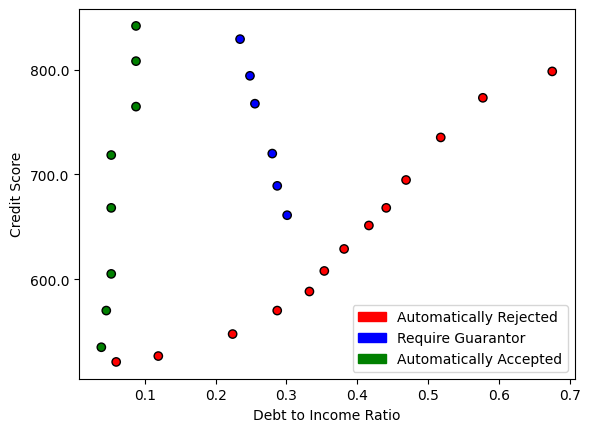
\includegraphics[width=.5\textwidth]{img_input/credit.png}
\end{center}
We've further transformed the raw data on debt to income ratio and credit score so that the default feature vector that you will be working with is defined as such:
\[\bm{x} = \left[\text{debt\_income\_ratio} \cdot \frac{200}{7}-7.5, \frac{\text{credit\_score}-500}{140}+0.5\right]^\top\]

\noindent Please implement the following classifiers:


\begin{enumerate}[label=\alph*)]

  \item \textbf{A generative classifier with Gaussian class-conditional
          densities with a \textit{shared covariance} matrix} across all classes.
        Feel free to re-use your Problem 2 results.

  \item \textbf{Another generative classifier with Gaussian class-conditional densities , but now
          with a \textit{separate covariance} matrix} learned for each class. (Note:
        The staff implementation can switch between the two Gaussian generative classifiers with just a
        few lines of code.)

  \item \textbf{A multi-class logistic regression classifier} using the softmax activation function. In your implementation of gradient descent, \textbf{make sure to use L2 regularization} with regularization parameter $\lambda = 0.001$. Please also include a \emph{\textbf{bias term, but do not regularize it}}. Limit the number of iterations of gradient descent to 200,000, and set the learning rate to be $\eta = 0.001$.

  \item \textbf{Another multi-class logistic regression classifier} with the additional feature map:
  $$\phi(\bm x) = [\ln (x_1+10), x_2^2]^\top$$

  \item \textbf{A kNN classifier} in which you classify based on the $k = 1$ and $k = 5$ nearest neighbors and the following distance function: 
  \[\text{dist}(\boldsymbol{x}, \boldsymbol{x}') = (x_1 - x'_1)^2/9 + (x_2 - x'_2)^2\]
        where nearest neighbors are those with the smallest distances from a given point.

        Note 1: When there are more than two labels, no label may have the
        majority of neighbors.  Use the label that has the most votes among
        the neighbors as the choice of label.

        Note 2: The grid of points for which you are making predictions
        should be interpreted as our test space.  Thus, it is not necessary
        to make a test point that happens to be on top of a training point
        ignore itself when selecting neighbors.

\end{enumerate}

After implementing the above classifiers, complete the following exercises:
  \begin{enumerate}



      \item Plot the decision boundaries generated by each classifier for the dataset. Include them in your PDF.
            Identify the similarities and differences among the classifiers. What explains the differences---in particular, which aspects or properties of each model dictate the shape of its decision boundary?
    
      \item
    
            Consider a loan applicant with Debt to Income Ratio 0.32 and Credit Score 350. To which class does each classifier assign this applicant? Report the classification probabilities of this applicant for models (c) and (d).
            
            Interpret how each model makes its classification decision. What else should we, the modelers, be aware of when making predictions on a point “far” from our training data? \textbf{Your response should no be longer than 5 sentences.}

    \item
        Can you think of any ethical problem that might arise from using this classifier to make loan decisions? You may approach this from any angle you like. For instance, can you think of someone who might have a low credit score and high debt-to-income ratio that you believe should nonetheless be offered a loan? Are there other variables that should be accounted for to ensure fair decisions? Are credit scores and debt-to-income ratio good bases for loan decisions? More generally, is using a classifier trained on past decisions to determine loan eligibility problematic in any way?
    \end{enumerate}
\end{problem}

\newpage

\begin{solution}
	\begin{enumerate}
	    \item \ \\ 
\includegraphics[width = 0.5\linewidth]{hw2/img_output/Gaussian Generative Classifier - Shared Covariance.png} 
\includegraphics[width = 0.5\linewidth]{hw2/img_output/Gaussian Generative Classifier - Seperate Covariance.png} \\
        
\includegraphics[width = 0.5\linewidth]{hw2/img_output/Softmax Regression.png} 
\includegraphics[width = 0.5\linewidth]{hw2/img_output/Softmax Regression - Feature Map.png} \\ 
\includegraphics[width = 0.5\linewidth]{hw2/img_output/KNN Classifier - k = 1.png} 
\includegraphics[width = 0.5\linewidth]{hw2/img_output/KNN Classifier - k = 5.png}\\
        The similarities are that almost all classifiers agree that low debt to income ratio and high credit score leads to acceptance, opposite to rejection, and something in between requires a guarantor. \\
        For differences, GGC with separate covariance, which doesn't really have a clear guarantor case and in its place is automatic rejection except for a small part of the graph. Both GGC with separate covariance and softmax reg with feature map have a part of the graph where low credit score and high debt to income ratio predicts guarantor, which should be automatic rejection. Softmax Reg w Feature Map, KNN = 5, and GGC w sep cov. automatically accept in low CS, high DtI ratio.\\
        GGC with shared cov's decision boundary shape is dictated by the shared covariance forcing all Gaussians to have identical shape with only centers differing, leading to linear boundaries.\\
        GGC with separate cov's decision boundary shape is dictated by the separate covariance allowing all Gaussians to have their own shape, leading to curved boundaries where the Gaussians are equally likely.\\
        Softmax Reg has linear boundaries because it computes linear scores, and softmax picks the highest score of those for the prediction.\\
        Softmax Reg w Feature map has curved boundaries because it computes scores in log and quadratic transformed space, and softmax creates linear boundaries in that space, which is non-linear in original space.\\
        KNN just uses the training data's nearest neighbors to create boundaries, and so they are curved spaces around the clusters for each class. KNN with k=5 allows more automatic accepts in places it shouldn't due to more training points of automatic accepts being more clustered together and automatic rejections being more spread out.
        \item Model a) prediction: [0], Model b) prediction: [0], Model c) prediction: [0], Model d) prediction: [1], KNN k=1 prediction: [0], KNN k=5 prediction: [0], Model c) probabilities: [[1. 0. 0.]], Model d) probabilities: [[0.254 0.659 0.087]].\\
        When making predictions on a point "far" from our training data, we must consider that the more complex models can produce undesired results in spaces outside of training data because of how their nonlinear boundaries can extend into those regions, like for model d). Since all models compute a score and then assign a probability, the distance from training data is not reflected in the prediction, so high confidence can be misleading if there is no data to support it.
        \item The problematic ethical aspect of such classifier is not accounting for social inequalities. For example, migrants and other minorities might not have as good access to credit as the general population, which puts them at a disadvantage. Special circumstances of a recent crisis despite ability to repay loan is also not reflected in this model. And more generally, training on past decisions, if they were biased, means that we translate this bias into our future predictions, so we have to be careful there.
        
	\end{enumerate}
\end{solution}

\newpage

\begin{problem}[Gradient Descent and Regularization, 15pts]

\noindent In this problem, you will analyze gradient descent for linear regression and study how \emph{ridge regularization} modifies the optimization landscape. You will first derive gradient descent updates for ordinary least squares, then extend them to the ridge-regularized objective. Finally, you will implement these algorithms to empirically observe how regularization affects convergence and generalization.

\medskip

\noindent Consider a regression dataset $\mathcal D = \{(\mathbf x_i, y_i)\}_{i=1}^N$, where each input $\mathbf x_i \in \mathbb{R}^D$ and response $y_i \in \mathbb{R}$. Let $\mathbf X \in \mathbb{R}^{N \times D}$ denote the design matrix and let $\mathbf y \in \mathbb{R}^N$ denote the vector of responses.
\\\\
\textbf{Detail:} The predictors in this dataset are \emph{highly correlated}.
As a result, the ordinary least squares objective may be ill-conditioned,
which can lead to unstable gradient descent updates and high-variance
parameter estimates. In later parts of this problem, we will examine how
ridge regularization modifies the optimization landscape in this setting.
\\\\
\noindent Consider the ordinary least squares objective
\begin{equation*}
    \mathcal L(\mathbf w) = \frac{1}{2} \|\mathbf X\mathbf w - \mathbf y\|_2^2.    
\end{equation*}

\begin{enumerate}

\item Derive the gradient $\nabla_{\mathbf w} \mathcal L(\mathbf w)$ with respect to the parameter vector $\mathbf w$. Your final expression should be written in matrix/vector form and simplified as much as possible.

\item Using your result, write the full-batch gradient descent update rule for
$\mathbf w$ with step size $\eta > 0$.
\\\\
\noindent Now consider the ridge-regularized objective
\begin{equation*}
    \mathcal L_\text{ridge}(\mathbf w) = \frac{1}{2} \|\mathbf X\mathbf w - \mathbf y\|_2^2 + \frac{\lambda}{2} \|\mathbf w\|_2^2,
\end{equation*}
where $\lambda \ge 0$ is a regularization parameter. Important note: typically, we do not regularize the bias term, $w_0$, thus $\|\mathbf w\|_2^2$ should be replace with $\mathbf w'$ where $w'_0 = 0$. However, for the sake of simplicity, we will omit that detail for the rest of the problem.

\item Derive the gradient $\nabla_{\mathbf w}\mathcal L_\text{ridge}(\mathbf w)$. Clearly indicate how the regularization term modifies the gradient compared to the unregularized case.


\item Rewrite the update in a form that makes the effect of ridge regularization
explicit. Briefly explain how this form illustrates the shrinkage effect of the
regularization term on the parameters.

\item You will implement gradient descent for both the ordinary least squares and
ridge-regularized objectives derived above and empirically study the effect of
regularization. Specifically, you will

\begin{itemize}
    \item Implement gradient and loss functions for both regular and ridge regression
    \item Write update step functions for stochastic gradient descent, stochastic gradient descent + momentum, and Adam optimizer.
\end{itemize}

Try not to touch anything that is not in between ``\textit{sol}" and ``\textit{los}"!


\item Generate the contour plots for the trajectories of the three algorithms across both the regularized and non-regularized case. What do you notice about the speed of convergence as well as where the algorithms converge to? What do you notice about the geometry of the loss function?\\
\textit{Note: the graphing code will pause when the first descent converges, so we see that some will not converge. Also, you'll see a subspace for the optimum in the unregularized case since we have a non-full rank data matrix $\mathbf X$!}

\end{enumerate}
\end{problem}

\pagebreak

\begin{solution}
	\begin{enumerate}
	    \item $$\mathcal L(\mathbf w) = \frac{1}{2} \|\mathbf X\mathbf w - \mathbf y\|_2^2$$
        $$\nabla_{\mathbf w} \mathcal L(\mathbf w) = X^T(\mathbf X\mathbf w - \mathbf y)$$
        \item $$w^{t+1} = w^t - \eta\nabla_{\mathbf w} \mathcal L(\mathbf w^t)$$
        $$w^{t+1} = w^t - \eta X^T(\mathbf X\mathbf w ^t- \mathbf y)$$
        \item $$\mathcal L_\text{ridge}(\mathbf w) = \frac{1}{2} \|\mathbf X\mathbf w - \mathbf y\|_2^2 + \frac{\lambda}{2} \|\mathbf w\|_2^2$$
        $$\nabla_{\mathbf w}\mathcal L_\text{ridge}(\mathbf w) = X^T(\mathbf X\mathbf w ^t- \mathbf y) + \lambda w$$
        \item $$w^{t+1} = w^t - \eta X^T(\mathbf X\mathbf w ^t- \mathbf y) - \eta\lambda w^t$$
        $$w^{t+1} = (1 - \eta \lambda)w^t - \eta X^T(\mathbf X\mathbf w ^t- \mathbf y)$$
        Since $\eta>0, \lambda>0$, the update first shrinks the previous weights by a factor of $\lambda \eta$, and then applies the same gradient step update as we saw in the non-regularized version.
        \item[6.] \ \\ 
\includegraphics[width = \linewidth]{hw2/img_output/4.6.png}
	\end{enumerate}
\end{solution}


%%%%%%%%%%%%%%%%%%%%%%%%%%%%%%%%%%%%%%%%%%%%%
% Name and Calibration
%%%%%%%%%%%%%%%%%%%%%%%%%%%%%%%%%%%%%%%%%%%%%

\pagebreak
\textbf{Name}: Ondrej Vesely

\textbf{Collaborators and Resources}: 

\end{document}
